% please run using
% lualatex --shell-escape ...tex

\documentclass[11pt,aspectratio=169]{beamer}
\setbeamertemplate{navigation symbols}{}
\usepackage{background}
\usepackage{booktabs}
\usepackage{tikz, rotating}
\usetikzlibrary{automata, arrows}
\usetikzlibrary{shapes.geometric}
\usepackage{tikzsymbols}
\usepackage{tabularx}
\usepackage{wrapfig}

\usepackage{amsmath, amsfonts, rotating, wasysym}
\usepackage{mathtools}
\usepackage{stmaryrd}
\usepackage{bbm}
\newcommand{\dickm}[1]{\text{\boldmath ${#1}$}}
\definecolor{gray}{rgb}{0.5,0.5,0.5}
\definecolor{middlegray}{rgb}{0.75,0.75,0.75}
\definecolor{lightgray}{rgb}{0.8,0.8,0.8}
\definecolor{lightblue}{rgb}{0.5,0.6,1}
\definecolor{green4}{rgb}{.1,.5,.1}
\newcommand{\changefont}[3]{
\fontfamily{#1} \fontseries{#2} \fontshape{#3} \selectfont}

\usepackage{comment}
\usepackage{minted}
\setminted{encoding=utf-8}
\usepackage{fontspec}
%\setmainfont{dejavu-serif}
\setmonofont[Scale=0.85]{dejavu-sans}
%\setmainfont{FreeSerif}
%\setmonofont{FreeMono}
\usepackage{xcolor, graphics}
% ensure clickable/colored links in the PDF
\usepackage{hyperref}
\hypersetup{colorlinks=true, linkcolor=blue, urlcolor=blue, citecolor=blue}
\definecolor{mygray}{rgb}{0.97,0.97,0.97}
\definecolor{LightCyan}{rgb}{0.8784,1,1}
\newcommand{\leanline}[1]{\mintinline[breaklines, breakafter=_., breaklines]{Lean}{#1}}%\textsuperscript{\textcolor{gray}{\tiny(m)}}}
\newcommand{\leanlinecolor}{\mintinline[breaklines, breakafter=_., breaklines, bgcolor=LightCyan]{Lean}}
\newcommand{\leanlogo}{\raisebox{-0.08cm}{
\includegraphics[height=0.5cm]{lean_logo.png}}}
\usepackage{refcheck}


%% ------------------------- document -------------------------------%

\title{Formalizing Probability Theory using the Lean Interactive Theorem Prover}
\author{Peter Pfaffelhuber}
\date{Frankfurt, May 13th, 2026}

\setbeamertemplate{blocks}[rounded][shadow=true]
\definecolor{darkgreen}{rgb}{0.0,0.4,0.0}
\definecolor{darkblue}{rgb}{0.1,0.1,0.5}
\definecolor{darkred}{rgb}{0.5,0.0,0.0}
\definecolor{middle_magenta}{rgb}{0.8,0.0,0.8}
\definecolor{middle_blue}{rgb}{0.0,0.0,0.8}
\definecolor{middle_red}{rgb}{0.8,0.0,0.0}
\definecolor{middle_green}{rgb}{0.0,0.6,0.0}
\definecolor{olive}{rgb}{0.44,0.4,0.05}
\definecolor{gray}{rgb}{0.35,0.35,0.35}
\setbeamercolor{title}{fg=white}
\setbeamercolor{author}{fg=white}
\setbeamercolor{date}{fg=white}

\begin{document}

\backgroundsetup{scale=1, color=black, opacity=1, angle=0, contents={\vspace*{3cm}\hspace*{-10cm}
\includegraphics[width=1.80\paperwidth,height=1.33\paperheight]{hintergrund_vortrag1.pdf}}}

\setbeamertemplate{background}{\BgMaterial}
\begin{frame}
  \titlepage
  
\end{frame}


% Content slides: no background image, small UFR logo as footer.
\setbeamertemplate{background}{}
\setbeamertemplate{footline}{%
  \hbox{\hskip 0.5cm
\includegraphics[height=0.55cm]{ufr.png}\hfill}%
  \vskip 4pt%
}

% \begin{frame}
%   \frametitle{}
%   \begin{enumerate}
%   \item {\bf Some history}
%
%     ~~
%
%   \item Short introduction to Lean
%
%   ~~
%
%   \item Discrete Probability in Lean
%
%   ~~
%
%   \item Brownian Motion in Lean
%
%   ~~
%
%   \item Changing the workflow of mathematics
%   \end{enumerate}
%
% \end{frame}

\begin{frame}
  \frametitle{Some \leanlogo{} pioneers}

  \vspace{0.5em}

  \begin{minipage}[t]{0.24\textwidth}
    \centering
    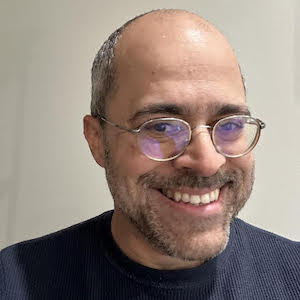
\includegraphics[height=2.2cm,keepaspectratio]{leo.jpg}\\[1ex]
    {\bf Leonardo di Moura}\\[0.2em]
    \small started Lean in 2013 at Microsoft.
  \end{minipage}\hfill
  \begin{minipage}[t]{0.24\textwidth}
    \centering
    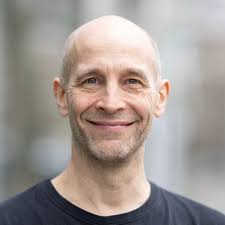
\includegraphics[height=2.2cm,keepaspectratio]{buzzard.jpeg}\\[1ex]
    {\bf Kevin Buzzard}\\[0.2em]
    \small promotes Lean for mathematicians since 2018.
  \end{minipage}\hfill
  \begin{minipage}[t]{0.24\textwidth}
    \centering
    
\includegraphics[height=2.2cm,keepaspectratio]{johan.jpg}\\[1ex]
    {\bf Johan Commelin}\\[0.2em]
    \small led the Liquid Tensor Experiment.
  \end{minipage}\hfill
  \begin{minipage}[t]{0.24\textwidth}
    \centering
    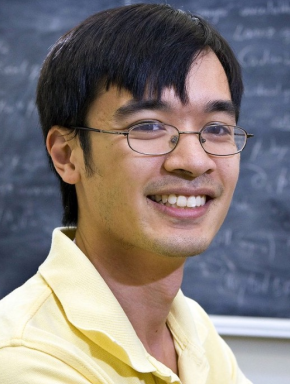
\includegraphics[height=2.2cm,keepaspectratio]{tao1.png}\\[1ex]
    {\bf Terrence Tao}\\[0.2em]
    \small leads collaborative formalization efforts.
  \end{minipage}
\end{frame}

% \begin{frame}
%   \frametitle{Harmonic}
%   \begin{minipage}[t]{2.5cm}
%     \vspace{0pt}
%     
\includegraphics[width=2cm]{harmonic.png}
%   \end{minipage}
%   \hfill
%   \begin{minipage}[t]{8cm}
%     \vspace{0pt}
%     Three AI-systems won Gold meadals (all with 5 out of 6 correct solutions):
%     \begin{itemize}
%     \item OpenAI: Solutions in natural language, general methods
%     \item Google DeepMind: Solutions in natural language, special mathematical methods
%     \item Harmonic: Solutions in Lean4, no human checks of solutions necessary.
%     \end{itemize}
%   \end{minipage}
% \end{frame}

\begin{frame}
  \frametitle{\leanlogo{}}

  \begin{itemize}
  \item Lean is a functional programming language.
  \item Developed by the Lean FRO ($\approx 20$ people).
  \item Key features: meta-programming, interactive theorem proving.
  \item The largest \href{https://leanprover-community.github.io/mathlib4_docs/mathlib.html}{mathematical library} is {\tt mathlib}, with about $2\cdot 10^6$ lines of code.
  \item The graphic shows the import structure of {\tt mathlib}.
  \end{itemize}

  \vfill
  \hfill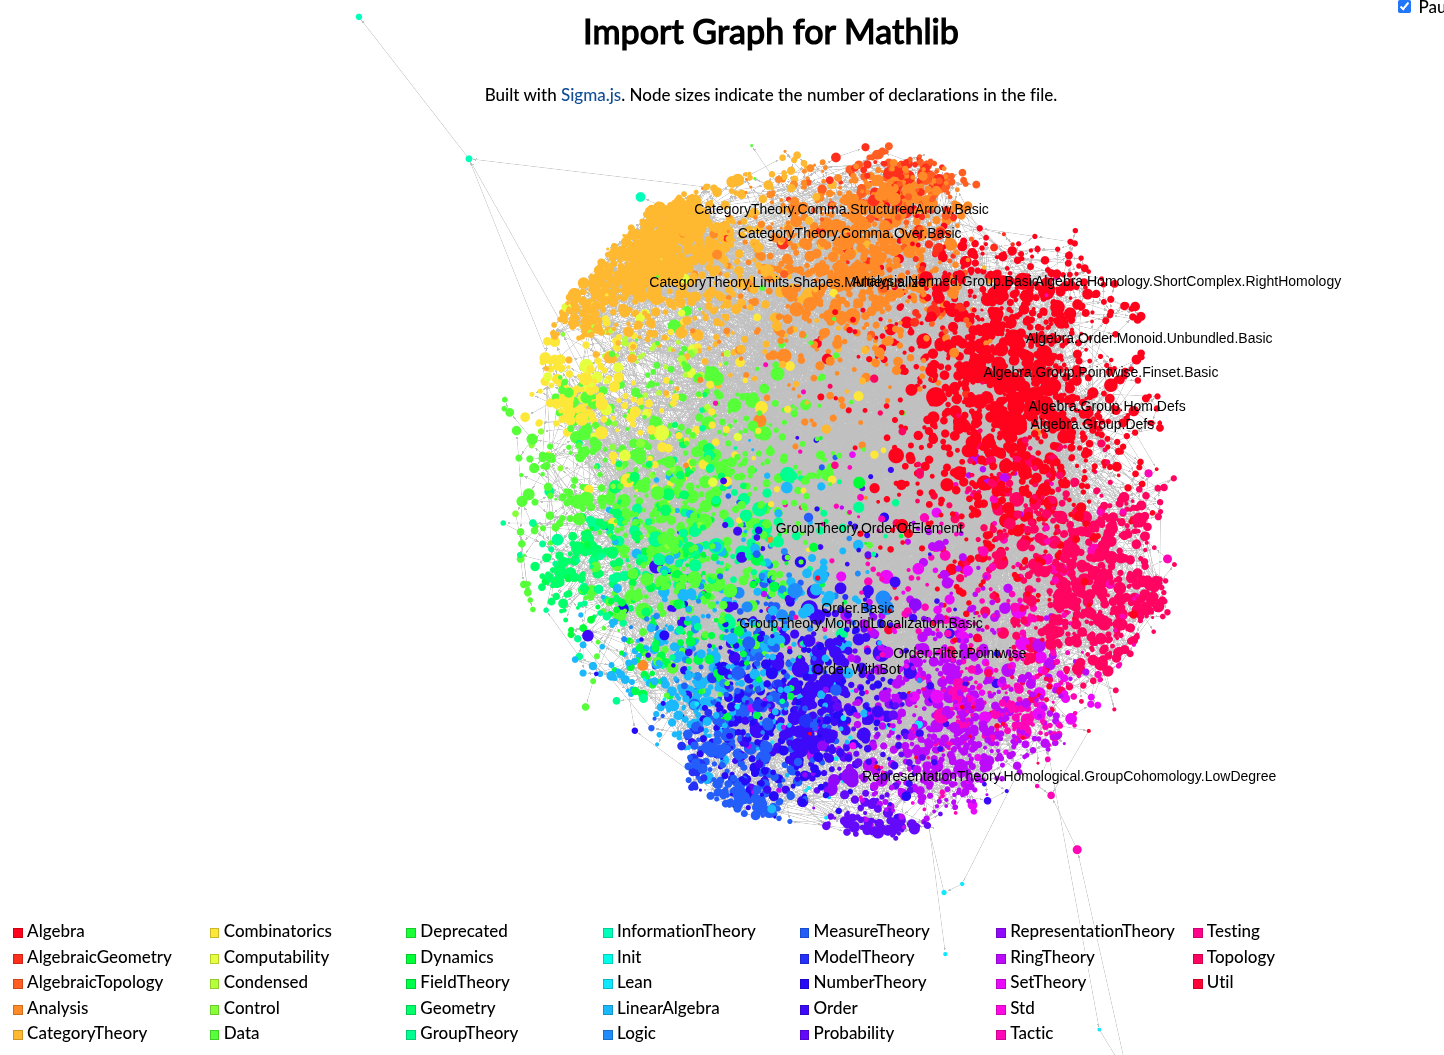
\includegraphics[trim=280 200 280 130,clip,height=2.8cm]{import.png}
\end{frame}

% \begin{frame}
%   \frametitle{}
%   \begin{enumerate}
%   \item Some history
%
%     ~~
%
%   \item {\bf Short introduction to Lean}
%
%   ~~
%
%   \item Discrete Probability in Lean
%
%   ~~
%
%   \item Brownian Motion in Lean
%
%     ~~
%
%   \item Changing the workflow of mathematics
%   \end{enumerate}
%
% \end{frame}

\begin{frame}
  \frametitle{\leanlogo{} demo}
  \begin{itemize}
    \item Divisibility

    ~~

    \item Unintuitive behavior
  \end{itemize}
\end{frame}

\begin{frame}
  \frametitle{\leanlogo{}}
  \begin{itemize}
  \item Every {\em term} has a {\em type}, e.g.:\\ \leanline{n : ℕ} or \leanline{α : Type} or \\
    \leanline{negneg_of_classical (p : Prop) : (p ∨ ¬ p) → (p ↔ ¬¬ p)}
  \item 
    There is a hierarchy of types: \leanline{Type 0} has type \leanline{Type 1} (in order to avoid logical pitfalls).
  \item Every type can be constructed, e.g.: \\
    \leanline{inductive ℕ where}\\
    \leanline{| zero : ℕ }\\
    \leanline{| succ (n : ℕ) : ℕ}    \\
    The construction of a \leanline{Prop}-type is its proof. 
  \end{itemize}

\end{frame}

\begin{frame}
  \frametitle{\leanlogo{}}

  \begin{itemize}
  \item Lean uses {\em dependent types}. Example: \\
  \leanline{  def Vec (α : Type) (n : ℕ) := { v : List α // v.length = n }}

    \vspace{-1.3cm}
    
    $$ \phantom{}\underbrace{\phantom{---------}}_{\text{Type Vec, which depends on the term $n : \mathbb N$}}\phantom{-------------------------------}$$

    Errors in the length of a {\tt Vec} are discovered at compile-time, not at run-time.


    ~

  \item[]
    \begin{center}
      Successful compilation of a lean file\\
      $\iff$\\
      all proofs in that file are correct.
    \end{center}

    ~

  \item The Curry-Howard isomorphism is described as {\em proofs-as-programs} and {\em propositions-as-types}. Example:\\
    \leanline{∀ x : Type*, x = x := fun x => rfl}
    
  \end{itemize}

\end{frame}

% \begin{frame}
%   \frametitle{}
%   \begin{enumerate}
%   \item Some history
%
%     ~~
%
%   \item Short introduction to Lean
%
%   ~~
%
%   \item {\bf Discrete Probability in Lean}
%
%   ~~
%
%   \item Brownian Motion in Lean
%
%     ~~
%
%   \item Changing the workflow of mathematics
%   \end{enumerate}
%
% \end{frame}

\begin{frame}[fragile]
  \frametitle{Discrete Probability}
  \begin{minted}[highlightlines={}, mathescape, numbersep=5pt, framesep=5mm, bgcolor=mygray]{Lean}
  structure DiscreteMeasure (α : Type*) where
    weight : α → ℝ≥0∞
  \end{minted}

  \vfill

  \begin{minted}[highlightlines={}, mathescape, numbersep=5pt, framesep=5mm, bgcolor=mygray]{Lean}
  noncomputable def toMeasure [MeasurableSpace α] :
    DiscreteMeasure α → Measure α :=
    fun μ ↦ Measure.sum (fun a ↦ μ.weight a • Measure.dirac a)
  \end{minted}

  \vfill

  \begin{minted}[highlightlines={}, mathescape, numbersep=5pt, framesep=5mm, bgcolor=mygray]{Lean}
  noncomputable def coin (p : unitInterval) :
      DiscreteMeasure Bool where
    weight
    | true  => ↑p
    | false => ↑(1 - p)
  \end{minted}
\end{frame}

\begin{frame}[fragile]
  \frametitle{Discrete Probability}
  \begin{minted}[highlightlines={}, mathescape, numbersep=5pt, framesep=5mm, bgcolor=mygray]{Lean}
  noncomputable def binom (p : unitInterval) :
      ℕ → DiscreteMeasure ℕ
    | 0 => dirac 0
    | n + 1 => do
      let X ← coin p
      let Y ← binom p n
      return (↑X + Y)
  \end{minted}
  \begin{minted}[highlightlines={}, mathescape, numbersep=5pt, framesep=5mm, bgcolor=mygray]{Lean}
  theorem binom_eq_count_true (p : unitInterval) (n : ℕ) :
      binom p n = do
        let X ← iidSequence n (coin p)
        return X.count true
  \end{minted}
\end{frame}

\begin{frame}
  \frametitle{Random variables}

  \begin{center}
    
\includegraphics[width=0.85\textwidth,height=0.38\textheight,keepaspectratio]{Kersting_RandVar.png}

    \vspace{0.5em}

    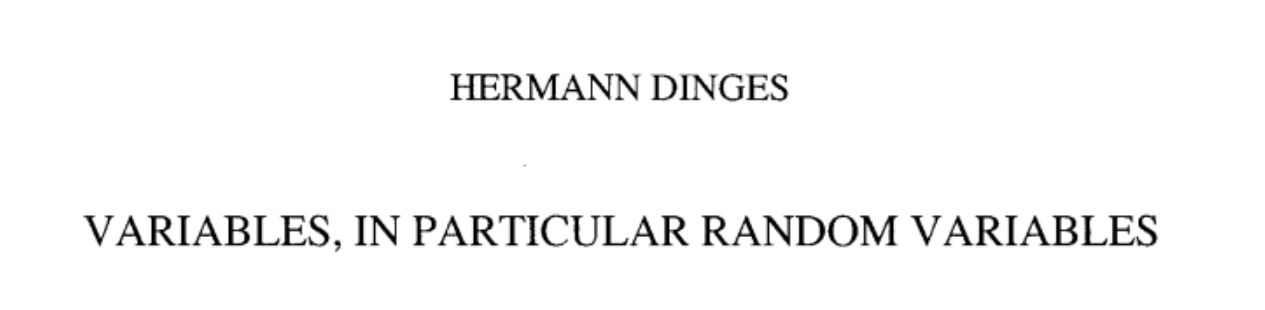
\includegraphics[width=0.85\textwidth,height=0.38\textheight,keepaspectratio]{Dinges_RandVar.png}
  \end{center}
\end{frame}

\begin{frame}[fragile]
  \frametitle{The probability monad}

  \begin{itemize}
  \item $\mathrm{DiscreteMeasure}\,\alpha$ \;=\; discrete probability measures on $\alpha$.
  \item $\mathrm{dirac}_\alpha : \alpha \to \mathrm{DiscreteMeasure}\,\alpha,\quad x \mapsto \delta_x$.
  \item A \emph{Markov kernel} $\kappa : \alpha \to \mathrm{DiscreteMeasure}\,\beta$ extends to
    $$\texttt{bind}\,\kappa : \mathrm{DiscreteMeasure}\,\alpha \to \mathrm{DiscreteMeasure}\,\beta.$$
  \end{itemize}

  \smallskip

  For $\kappa : \alpha \to \mathrm{DiscreteMeasure}\,\beta$, $\eta : \beta \to \mathrm{DiscreteMeasure}\,\gamma$:
  \begin{align*}
    \texttt{bind}\,(\mathrm{dirac}_\alpha)\,\mu \;&=\; \mu && %\text{(returning $\delta_X$ for $X \sim \mu$ averages back to $\mu$)} 
    \\
    \texttt{bind}\,\kappa\,(\delta_x) \;&=\; \kappa(x) && % \text{(deterministic input gives kernel output)} 
    \\
    \texttt{bind}\,(\texttt{bind}\,\eta \circ \kappa) \;&=\; \texttt{bind}\,\eta \circ \texttt{bind}\,\kappa && \text{(Chapman--Kolmogorov)}
  \end{align*}
  Pushforward and mixture are derived from \texttt{dirac} and \texttt{bind}:
  \begin{align*}
    \texttt{map}\,f \;&=\; \texttt{bind}\,(\mathrm{dirac} \circ f) && \text{(for $f : \alpha \to \beta$; law of $f(X)$ for $X \sim \mu$)} \\
    \texttt{join} \;&=\; \texttt{bind}\,\mathrm{id} && \text{(average over a random measure $\Xi \sim m$)}
  \end{align*}
\end{frame}

\begin{comment}
\begin{frame}[fragile]
  \frametitle{The probability monad}

  The \leanline{do}-notation definition of \leanline{binom} is definitionally
  equal to a sequence of \leanline{bind}s and \leanline{pure}:

  \begin{minted}[highlightlines={}, mathescape, numbersep=5pt, framesep=5mm, bgcolor=mygray]{Lean}
  noncomputable def binom (p : unitInterval) :
      ℕ → DiscreteMeasure ℕ
    | 0 => dirac 0
    | n + 1 => do
      let X ← coin p
      let Y ← binom p n
      return (↑X + Y)
  \end{minted}

  \begin{minted}[highlightlines={}, mathescape, numbersep=5pt, framesep=5mm, bgcolor=mygray]{Lean}
    theorem binom_succ (p : unitInterval) (n : ℕ) :
      binom p (n + 1) =
        (coin p).bind (fun X => (binom p n).bind 
          (fun Y => pure (X.toNat + Y)))
    := rfl

  \end{minted}
\end{frame}
\end{comment}

\begin{frame}[fragile]
  \frametitle{The probability monad}

  \begin{itemize}
  \item \leanline{dirac a} = Dirac measure $\delta_a$.
  \item \leanline{μ.map f} = pushforward: law of $f(X)$ when $X \sim μ$.
  \item \leanline{Ξ.join} = mixture: average over a random measure $\mu \sim \Xi$.
  \item \leanline{μ.bind f} = sample $X \sim μ$, then $Y \sim f(X)$.
  \end{itemize}

  \begin{minted}[highlightlines={}, mathescape, numbersep=5pt, framesep=5mm, bgcolor=mygray]{Lean}
  noncomputable def map (g : α → β) (μ : DiscreteMeasure α) :
      DiscreteMeasure β :=
    ⟨fun b ↦ ∑' a, (g⁻¹' {b}).indicator μ.weight a⟩

  noncomputable def join (Ξ : DiscreteMeasure (DiscreteMeasure α)) :
      DiscreteMeasure α :=
    ⟨fun a ↦ ∑' μ, Ξ μ * μ a⟩

  noncomputable def bind (μ : DiscreteMeasure α)
      (f : α → DiscreteMeasure β) : DiscreteMeasure β :=
    (μ.map f).join
  \end{minted}
\end{frame}

\begin{frame}[fragile]
  \frametitle{The probability monad}

  These operations satisfy the monad laws, the most involved being
  associativity of \leanline{bind}:

  \begin{minted}[highlightlines={}, mathescape, numbersep=5pt, framesep=5mm, bgcolor=mygray]{Lean}
  theorem bind_bind (μ : DiscreteMeasure α)
      (f : α → DiscreteMeasure β) (g : β → DiscreteMeasure γ) :
      (μ.bind f).bind g = μ.bind (fun a ↦ (f a).bind g)
  \end{minted}

  \begin{minted}[highlightlines={}, mathescape, numbersep=5pt, framesep=5mm, bgcolor=mygray]{Lean}
  instance : LawfulMonad DiscreteMeasure
  \end{minted}

  This unlocks \leanline{do}-notation, which desugars to nested binds:

  \begin{minted}[highlightlines={}, mathescape, numbersep=5pt, framesep=5mm, bgcolor=mygray]{Lean}
  do
    let X ← μ
    let Y ← ν
    return (f X Y)
  -- is the same as
  μ.bind (fun X ↦ ν.bind (fun Y ↦ dirac (f X Y)))
  \end{minted}
\end{frame}

\begin{frame}
  \frametitle{Discrete Probability (Insights from formalization)}
  \begin{itemize}
  \item Discrete probability theory is like probability theory without any measurability issues.\\
  (This makes discrete probability measures a lawful monad.)
  \item Using \leanline{do}-Notation requires use of monads, and make definitions more readable.
  \item The binomial distribution can be defined in several equivalent ways. 
  \item Formalizing basic mathematics already feels like developing a theory. 
  \item Mathematically easy things can be hard to prove formally. \\
    (Equivalence of all definitions of the binomial distribution.)
\end{itemize}

\end{frame}

% \begin{frame}
%   \frametitle{}
%   \begin{enumerate}
%   \item Some history
%
%     ~~
%
%   \item Short introduction to Lean
%
%   ~~
%
%   \item Discrete Probability in Lean
%
%   ~~
%
%   \item {\bf Brownian Motion in Lean}
%
%     ~~
%
%   \item Changing the workflow of mathematics
%   \end{enumerate}
%
% \end{frame}

\begin{frame}[fragile]
  \frametitle{Submitted Dec 1st, 2025}
  \centering
  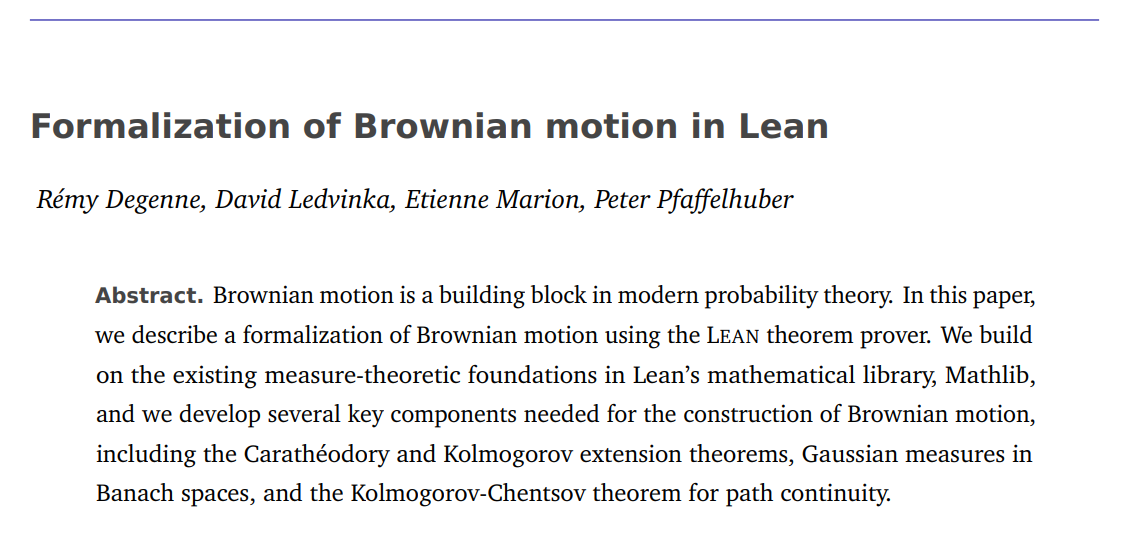
\includegraphics[width=0.85\textwidth,height=0.82\textheight,keepaspectratio]{BM.png}
\end{frame}

% \begin{frame}
%   \frametitle{}
%   \begin{enumerate}
%   \item Some history
%
%     ~~
%
%   \item Short introduction to Lean
%
%   ~~
%
%   \item Discrete Probability in Lean
%
%   ~~
%
%   \item Brownian Motion in Lean
%
%     ~~
%   \item {\bf Changing the workflow of mathematics}
%   \end{enumerate}
%
% \end{frame}
\end{document}

\begin{frame}[fragile]
  \frametitle{Brownian Motion (History of the project)}
  \begin{itemize}
  \item In 2023, Rémy Degenne (INRIA Lille) and I formalized the Kolmogorov Extension Theorem: 
  
  \begin{quote}
  A family $(P_J)_{J \subseteq_f I}$ of probability measures on $E_J$ for $J \subseteq_f I$, is projective if for
  all $H \subseteq J \subseteq_f I$, the pushforward $(\pi_H^J)_\ast P_J = P_H$. \\
  Extension theorem: a projective family $(P_J)_{J \subseteq_f I}$ defines a unique measure $E^I$ whose finite dimensional marginals are the $P_J$'s.
  \end{quote}
  \item The paper was rejected, the project was stuck, but we wanted to formalize Brownian Motion. 
  \item Rémy suggested to make a \href{https://remydegenne.github.io/brownian-motion/blueprint/}{collaborative project}. This worked very well and was finished in only a few weeks.
  \end{itemize}

\end{frame}

\begin{frame}
  \frametitle{Brownian Motion (Construction overview)}
  \begin{itemize}
  \item Implement characterstic functions \\ (in order to characterize Gaussian measures)
  \item Build multivariate Gaussians \\ (only Gaussians on $\mathbb R$ in Mathlib at the time)
  \item Prove that the Gaussian family with Covariance $s \wedge t$ exists and is projective.
  \item Use the Kolmogorov extension theorem in order to have a stochastic process with correct fdds. 
  \item Implement the Kolmogorov-Chentsov continuity theorem in a modern version for general index sets \\ (Krätschmer \& Urusov, 2023).
  \item Use the Kolmogorov-Chentsov continuity theorem to get a modification with continuous paths. 
  \end{itemize}

\end{frame}

\begin{frame}[fragile]
  \frametitle{Brownian Motion 1 (Kolmogorov extension)}
  \begin{minted}[highlightlines={}, mathescape, numbersep=5pt, framesep=5mm, bgcolor=mygray]{Lean}
noncomputable def kolmogorovExtension {ι : Type*} 
  {α : ι → Type*} {P : ∀ J : Finset ι, Measure (Π j : J, α j)} 
  [∀ i, PseudoEMetricSpace (α i)] [∀ i, BorelSpace (α i)] 
  [∀ i, SecondCountableTopology (α i)] [∀ i, CompleteSpace (α i)] 
  (P : ∀ J : Finset ι, Measure (Π j : J, α j)) [∀ i, IsFiniteMeasure (P i)] 
  (hP : IsProjectiveMeasureFamily P) : Measure (Π i, α i) := ...
\end{minted}
\end{frame}

\begin{frame}[fragile]
  \frametitle{Brownian Motion 2 (Kolmogorov-Chentsov Theorem)}
  \begin{minted}[highlightlines={}, mathescape, numbersep=5pt, framesep=5mm, bgcolor=mygray]{Lean}
/-- A stochastic process `X : T → Ω → E` on an index space `T` and 
a measurable space `Ω` with measure `P` is said to satisfy the 
Kolmogorov condition with exponents `p, q` and constant `M` if for 
all `s, t : T`, the pair `(X s, X t)` is measurable for the Borel 
sigma-algebra on `E × E` and the following condition holds: 
`∫⁻ ω, edist (X s ω) (X t ω) ^ p ∂P ≤ M * edist s t ^ q`. -/
structure IsKolmogorovProcess (X : T → Ω → E) (P : Measure Ω) 
  (p q : ℝ) (M : ℝ≥0) : Prop where
    measurablePair : ∀ s t : T, Measurable[_, borel (E × E)] 
      fun ω ↦ (X s ω, X t ω)
    kolmogorovCondition : ∀ s t : T, 
      ∫⁻ ω, edist (X s ω) (X t ω) ^ p ∂P ≤ M * edist s t ^ q
    p_pos : 0 < p
    q_pos : 0 < q
  \end{minted}
\end{frame}

\begin{frame}[fragile]
  \frametitle{Brownian Motion 3 (Continuous modification)}

  \begin{minted}[highlightlines={}, mathescape, numbersep=5pt, framesep=5mm, bgcolor=mygray]{Lean}
-- A stochastic process is called **pre-Brownian** if its finite-
dimensional laws are those of a Brownian motion, see 
`gaussianProjectiveFamily`. -/
class IsPreBrownian (P : Measure Ω := by volume_tac) : Prop where
  mk' ::
  hasLaw : ∀ I : Finset ℝ≥0, HasLaw (fun ω ↦ I.restrict (X · ω)) 
    (gaussianProjectiveFamily I) P
  \end{minted}
  \begin{minted}[highlightlines={}, mathescape, numbersep=5pt, framesep=5mm, bgcolor=mygray]{Lean}
noncomputable def gaussianProjectiveFamily (I : Finset ℝ≥0) :=
  multivariateGaussian 0 (brownianCovMatrix I) |>.map 
    (MeasurableEquiv.toLp 2 (I → ℝ)).symm
  \end{minted}
  \begin{minted}[highlightlines={}, mathescape, numbersep=5pt, framesep=5mm, bgcolor=mygray]{Lean}
/-- A stochastic process is called **Brownian** if its finite-
dimensional laws are those of a Brownian motion, see 
`IsPreBrownian`, and if it has almost-sure continuous paths. -/
class IsBrownian (X) (P : Measure Ω := by volume_tac) : 
  Prop extends IsPreBrownian X P where
    cont : ∀ᵐ ω ∂P, Continuous (X · ω)
  \end{minted}
\end{frame}

\begin{frame}[fragile]
  \frametitle{Brownian Motion 4 (The definition)}
  \begin{minted}[highlightlines={}, mathescape, numbersep=5pt, framesep=5mm, bgcolor=mygray]{Lean}
/-- If `h : IsPreBrownian X P`, then `h.mk X` is a continuous 
modification of `X`. -/
protected noncomputable def IsPreBrownian.mk (X) 
  [h : IsPreBrownian X P] : ℝ≥0 → Ω → ℝ :=
  h.exists_continuous_modification.choose
  \end{minted}
  \begin{minted}[highlightlines={}, mathescape, numbersep=5pt, framesep=5mm, bgcolor=mygray]{Lean}
noncomputable
def brownian : ℝ≥0 → (ℝ≥0 → ℝ) → ℝ := 
  isPreBrownian_preBrownian.mk
  \end{minted}
\end{frame}

\begin{frame}
  \frametitle{Brownian Motion (Insights from formalization)}
  \begin{itemize}
  \item Kolmogorov extension theorem does not require the same space $E$ at all time points. 
  \item Sometimes constants in paper proofs are wrong; they are easy to fix in Lean.
  \item Often, results can be generalized from metric spaces to pseudo-metric spaces \\ (Kolmogorov extension, Kolmogorov-Chentsov).
  \item Measurability has to be taken more seriously when working in Lean.
  \item Collaborative formal projects are a new way of interaction between mathematicians.
\end{itemize}

\end{frame}

\begin{frame}
  \frametitle{Start: \href{https://adam.math.hhu.de/}{The Natural Number Game}}

  \parbox[t]{0.5\textwidth}{ 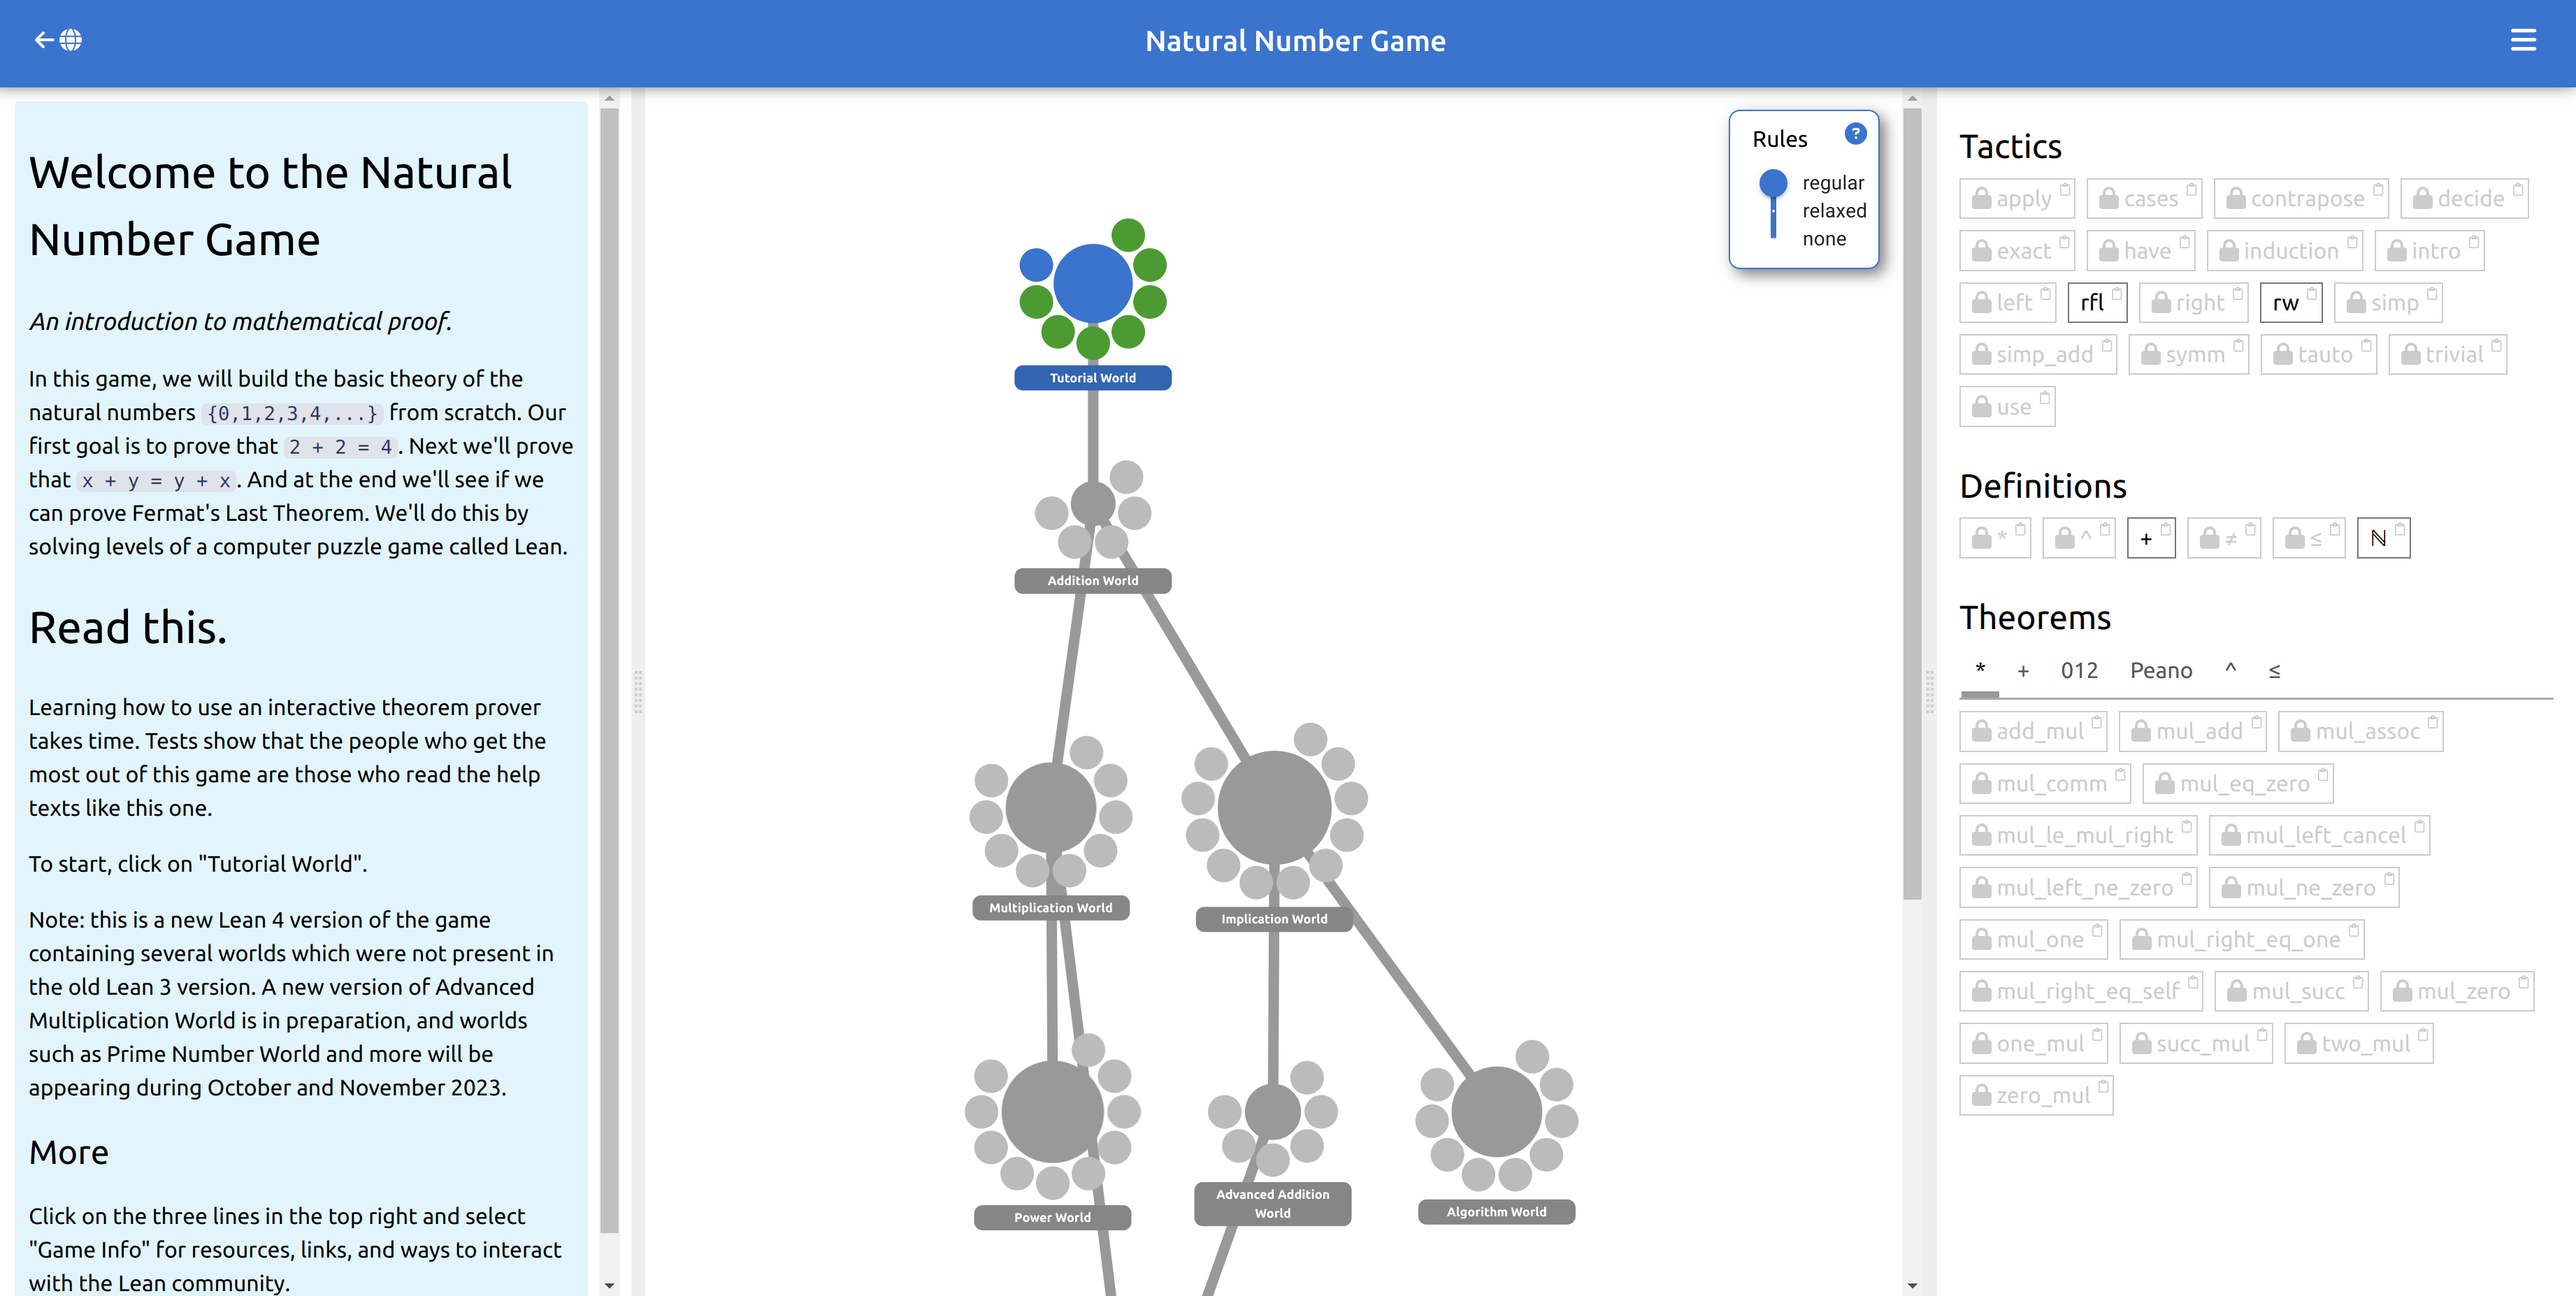
\includegraphics[width=\textwidth]{nng.png}}

\end{frame}



\end{document}


\begin{frame}
  \frametitle{}
  \begin{itemize}
    \item 
  \end{itemize}
\end{frame}

